%% Full length research paper template
%% Created by Simon Hengchen and Nilo Pedrazzini for the Journal of Open Humanities Data (https://openhumanitiesdata.metajnl.com)

\documentclass{article}
\usepackage[english]{babel}
\usepackage[utf8]{inputenc}
\usepackage{johd}
\usepackage{listings}
\usepackage{color}
\usepackage[demo]{graphicx}
\usepackage{subfig}
\usepackage{pythonhighlight}
\usepackage{array}

\definecolor{dkgreen}{rgb}{0,0.6,0}
\definecolor{gray}{rgb}{0.5,0.5,0.5}
\definecolor{mauve}{rgb}{0.58,0,0.82}

\lstset{frame=tb,
  language=HTML,
  aboveskip=3mm,
  belowskip=3mm,
  showstringspaces=false,
  columns=flexible,
  basicstyle={\small\ttfamily},
  numbers=none,
  numberstyle=\tiny\color{gray},
  keywordstyle=\color{blue},
  commentstyle=\color{dkgreen},
  stringstyle=\color{mauve},
  breaklines=true,
  breakatwhitespace=true,
  tabsize=3
}

\title{I Spy With My Little Pixel}

\author{Hayes Choy\\z5258816\\W19A - COMP6841}

\date{\today}

\begin{document}

\maketitle

\begin{abstract} 
\noindent My project is a proof of concept on how spy pixels can be used to track when the recipient of an email opens an email, and the user’s metadata. I have successfully created a backend to log all reads of a spy pixel, a database to store this data, and a frontend to create new spy pixels and view logs in a readable format. Furthermore, as a side project, I have learnt how HTML is used in emails, and investigated its differences with HTML in web development!
\\
\\
My spy pixel service is deployed at \href{https://spy-pixel.netlify.app}{\texttt{https://spy-pixel.netlify.app}} with the spy pixel itself being deployed at \href{https://spy-pixel.ts.r.appspot.com/spy-pixel.gif}{\texttt{https://spy-pixel.ts.r.appspot.com/spy-pixel.gif}}

\end{abstract}

\section{\label{context}Context and motivation}

\subsection{Email tracking}

If you've used a mass email service before, chances are the service also has a feature showing which recipients have read your email. Late last year and early this year, I was required to use GMass and was shocked when I could not only see the time they read my email, but also the number of unique clicks, replies and bounces.

\begin{figure}[H]
\centering
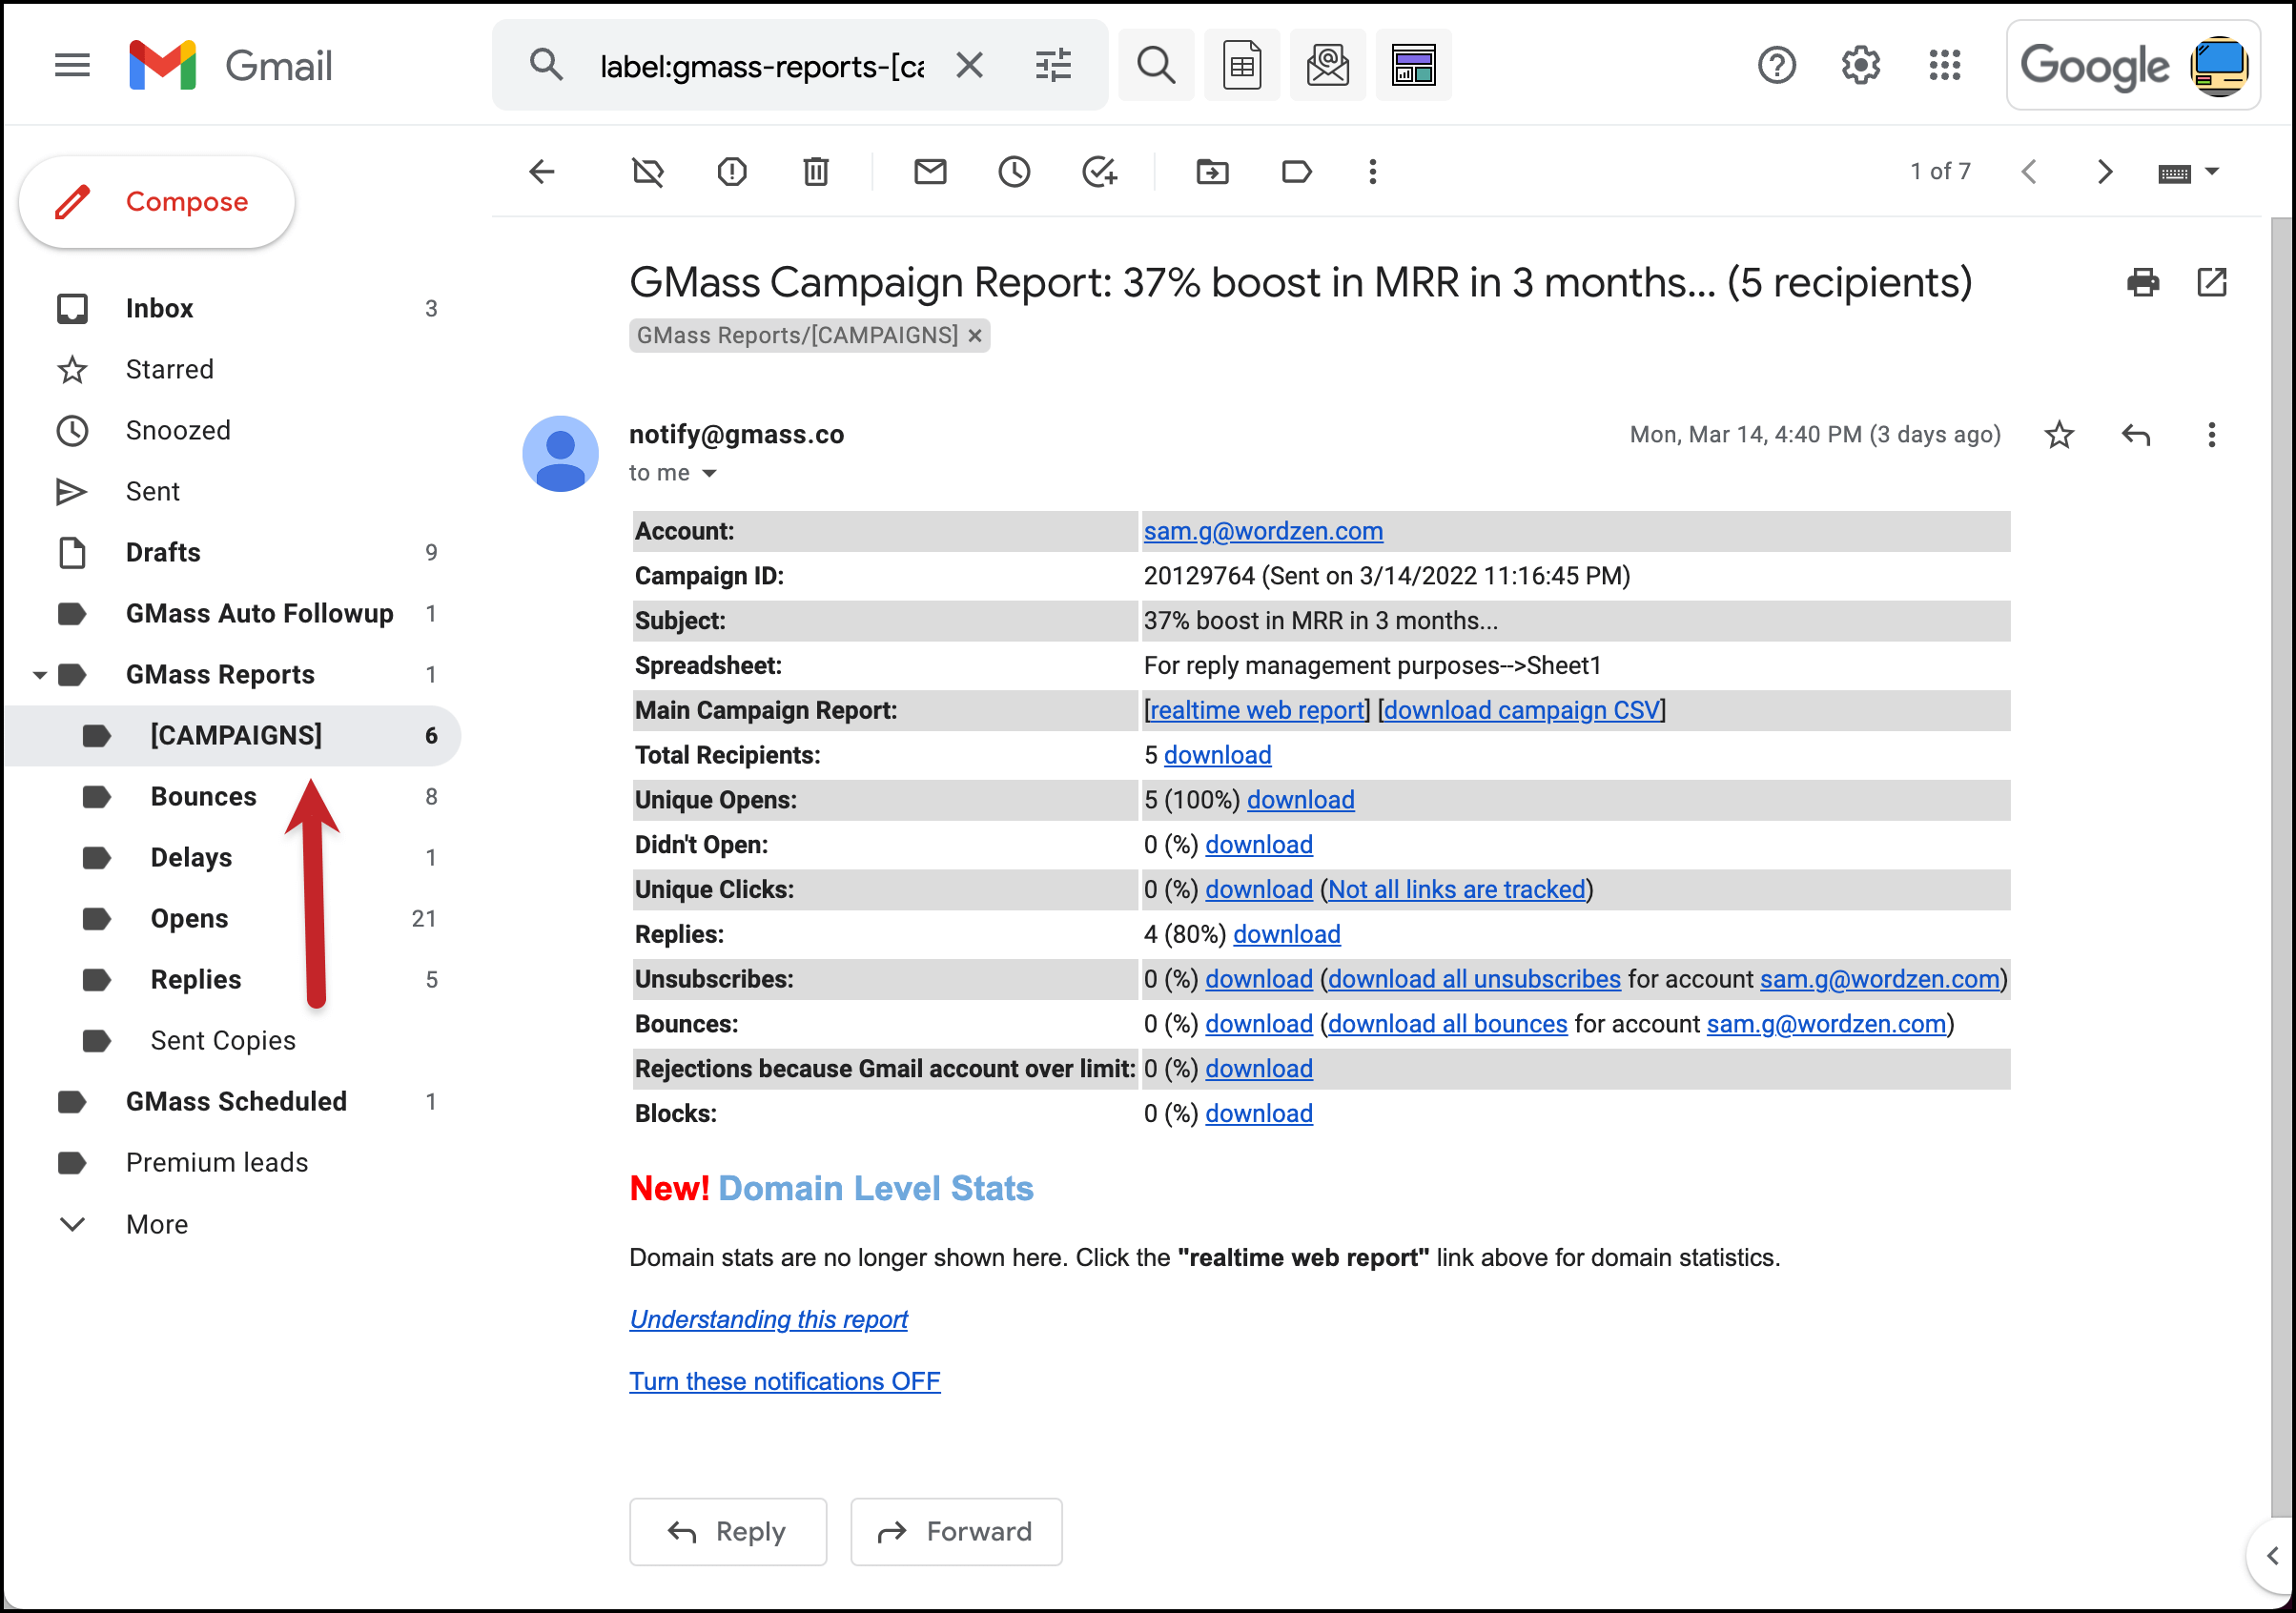
\includegraphics[width=0.8\textwidth]{images/gmass.png}
\caption{\label{fig1}GMass feature demo}
\end{figure}

Like Slack or old text messages, I had always assumed emails were a safe place where read receipts would never be implemented, and I could safely "seen" emails and procrastinate a reply. Clearly my assumptions were wrong, and for my project I wanted to understand how they worked, and perhaps, what other information I might be sending.

After a few Google searches, I learnt that this feature was made possible thanks to spy pixels.

\subsection{What is a spy pixel?}

A spy pixel is a 1x1 pixel transparent image that is sent alongside email content, with its source as an HTTP request to a server. When the email is loaded on the recipient's side, the transparent pixel image is sent from the server, and the request is logged by the server. It looks something like this:
\begin{lstlisting}
<img width="1" height="1" border="0" src="http://www.host.com/spy-pixel.png" />
\end{lstlisting}

The server is able to parse through the request headers and extract information about the user, such as their browser, device, OS, architecture and their location.

\subsection{Where are they used?}

Spy pixels are used \textbf{everywhere!}. On 10 March I opened up my inbox and inspected the elements of each email I received. Every newsletter seemed to contain a spy pixel embedded, to track whether I read it or not. Screenshots can be found in Appendix \ref{appendix-inbox} as examples.

From a marketing perspective, this makes sense. Marketers would be able to adapt their approach to their subscribers based on the activity collected from an email. If an email was able to prompt the user to read the email, click on its links, and then later lead to a purchase, then the email would be considered successful. As Richard Buckland says, "if data can be collected then it will be collected", and it seems that all digital newsletters now have this feature to better their interactions with customers.

\subsection{How to stop spy pixels}

The scary thing is that you \emph{can't} stop spy pixels from being embedded into emails. Spy pixels take advantage of the way HTML \texttt{img} tags fetch data from a host if the source isn't local, and this feature isn't always bad. This feature is what allows emails to have variety with its graphics, and removing this feature from email clients would force every email to be a boring black and white text.

Another point of concern is that the use of spy pixels are a grey area legally since the user isn't aware of the data being collected. However, that has never stopped companies from collecting data.

The only way to really stop these spy pixels from happening is to download an extension that pre-parses your email before rendering, and removes the spy pixel from HTML before showing it to the user. Examples include \href{https://chrome.google.com/webstore/detail/pixelblock/jmpmfcjnflbcoidlgapblgpgbilinlem?hl=en}{PixelBlock} or \href{https://chrome.google.com/webstore/detail/tracker-blocker-stop-trac/okacfeiojkgmcaonaikblpicellplcdn?hl=en}{Tracker Blocker}, but these are limited to web-based email clients and don't prevent spy pixels from appearing on your phone. They also tend to only work on popular email clients such as GMail or Outlook.

\begin{figure}[H]
\centering
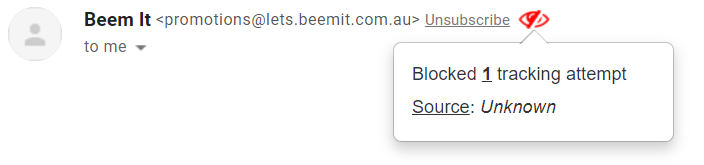
\includegraphics[width=0.8\textwidth]{images/beem.png}
\caption{\label{beem}PixelBlock blocking a spy pixel in an email from Beem It}
\end{figure}

While creating my own spy pixel service, I also discovered GMail's native approach to spy pixels. Each image rendered in an email is sent through GoogleImageProxy, which anonymises the user data. This prevented my spy pixel from detecting any of the user's metadata. So while a spy pixel is able to detect when a user has read an email, it is restricted to only do just that. Other email clients such as Outlook unfortunately don't go through the effort of anonymising user metadata. The proxy in the HTML looks like this:

\newpage

\begin{lstlisting}
<img border="0" width="1" height="1" src="<https://ci5.googleusercontent.com/proxy/wikffdoJfWk_6vlXa4vNaI-mb-CxwEvf
JyjqNqxh5QR_w8HUzTG56yLC1JuiTlgg7YSXnGilNh9N9U-dmosqVXjDYFNbDbYdgOf88nOZ_YeDqo
x3IBhvD0fmf34pzpsJ_zchN85j2WswRkd7TGLH=s0-d-e1-ft#https://fc78d80ff607aedccf6c
95947b81ab9f.tinyemails.com/f78c1d94d2d81b947af7fdde67b24818.gif>" />
\end{lstlisting}

It's important to note that it's the process of loading an image that makes a user trackable. Spy pixels have become the industry standard since they are super small, meaning they minimally affect load times, and are transparent, meaning the user won't notice them. However, any image that loads off an external server can be used, including email signatures or header banners! These aren't detected by the above Chrome extensions, so overall, it's virtually impossible to prevent the collection of your metadata as you browse your emails.

\subsection{What about clicks?}

Clicks are tracked using URL forwarders, such as Bitly or other URL shorterners. When a request is sent to a server, it redirects the browser to the actual link and logs the redirect. This is a fairly simple idea, and a service that is readily available, so this feature is not explored in this project's scope.

\section{Implementation of my spy pixel service}

\subsection{Backend}

My backend was created using Flask in Python 3 and is deployed on a Google Cloud App Engine instance. The main code responsible is in Appendix \ref{appendix-backend-code}.

The pixel is generated in the last three lines of the function. Since the image is of 1x1 pixel size, we can encode the image and store it as a hard-coded string. Thanks to the website \href{https://png-pixel.com}{\texttt{https://png-pixel.com}}, it gave me all the strings I needed. It turns out a GIF saves a few bytes, which would improve load performance, which is why I have decided on a \texttt{/spy-pixel.gif} route.

\begin{python}
gif_str = base64.b64decode('R0lGODlhAQABAIAAAP///////yH5BAEKAAEALAAAAAABAAEAAAICTAEAOw==')
\end{python}

When a request is called at the \texttt{/spy-pixel.gif} route, it first checks if the request came from the deployed service copying the spy pixel to the user's clipboard or is from when the user copy pastes it into their email. This is because both of these operations trigger a call to the backend, causing it to be logged. We don't want to log our own views, so we disregard either calls.

\begin{python}
if request.headers.get("Referer") != "https://mail.google.com/" and request.headers.get("Referer") != "https://spy-pixel.netlify.app/":
\end{python}

Since HTTP requests won't include the email address of the recipient, I needed to find a way to link the spy pixel with a recipient or a campaign. The neat thing about HTTP requests is that you can also provide query parameters, so my spy pixel is designed to store campaign IDs and emails in the URL. Campaign IDs are compulsory so that it has a point of reference and can summarise data from multiple spy pixels. Email identifiers are optional, but allow the sender to differentiate between recipients if they wish. If there is a campaign ID present in the request, then we log the data to the database.

\begin{lstlisting}
<img width="1" height="1" border="0" src="https://spy-pixel.ts.r.appspot.com/spy-pixel.gif?campaign=CAMPAIGNID&email=E@MAIL" />
\end{lstlisting}

\subsection{Database}

I used Firestore as my database. I chose Firestore since I've had experience using it before in my JavaScript projects and knew that the general functionality was easy to use. I also wanted to learn how to integrate it into Python projects, which I had never done before.

\subsection{Frontend}

The frontend (deployed at \href{https://spy-pixel.netlify.app}{\texttt{https://spy-pixel.netlify.app}}) has two types of pages: a dashboard, containing a spy pixel creator and ongoing campaigns, and a campaign details page.

\subsubsection{Spy Pixel Creator}

The spy pixel creator is the frontend interface to creating a spy pixel. A spy pixel can be easily created manually by writing some HTML and using a \texttt{img} tag, but I wanted to make this user friendly for not just coders! A spy pixel can take in two query parameters: the campaign ID and an optional email identifier. The copy to clipboard button is disabled until a valid campaign ID is entered. Also, since campaign IDs will be reused often, I added a datalist containing all the current campaign IDs so that the user can easily click on them if reusing a campaign ID.

\begin{figure}[H]
\centering
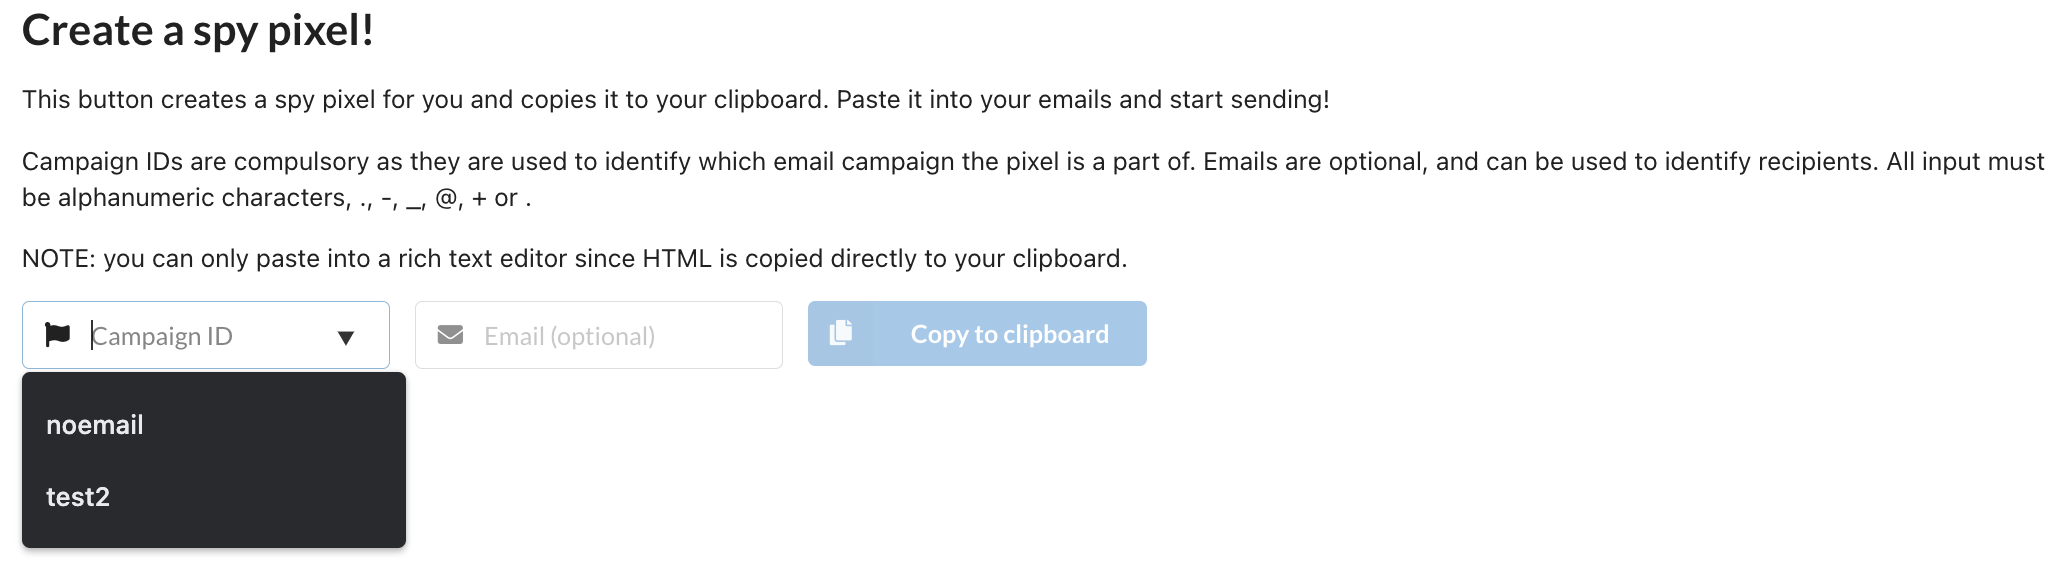
\includegraphics[width=0.8\textwidth]{images/create-spy-pixel.png}
\caption{Spy pixel creator with pre-loaded datalist}
\end{figure}

Upon clicking the copy to clipboard button, the image is rendered invisibly and then copied into the clipboard. This can then be pasted into a rich text editor such as an email draft, which would sit invisibly in the body content! A side effect of this method is that it triggers a render of the spy pixel, and sends a request to my backend. This is why my backend requires an \texttt{if} statement to ignore any requests referred from the frontend site. Unfortunately, this was the only way to get it to work since other methods would copy the HTML as plaintext and not as HTML.

\begin{figure}[H]
\centering
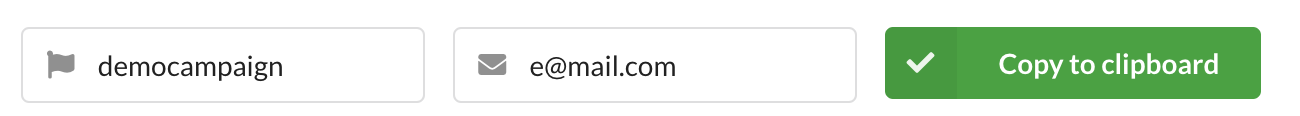
\includegraphics[width=0.8\textwidth]{images/copy-to-clipboard.png}
\caption{Responsive copy spy pixel to clipboard button}
\end{figure}

I also realised that since I was passing in a parameter straight into HTML, I was vulnerable to a XSS attack! If JavaScript was injected into the parameters, then the process of loading the image and copying it into the clipboard could trigger the script and run malicious code. To prevent this from happening, I disabled the copy to clipboard button if it detected characters that weren't on the whitelist, and visually showed which parameter was causing this error by highlighting the input box red.

\begin{figure}[H]
\centering
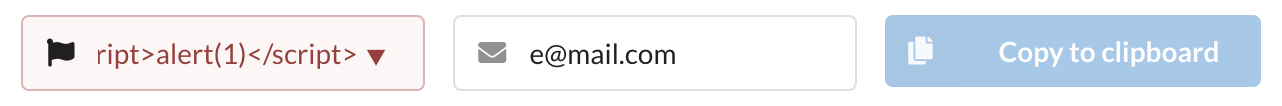
\includegraphics[width=0.8\textwidth]{images/xss-block.png}
\caption{Input boxes turn red on invalid input}
\end{figure}

\subsubsection{List of campaigns}

Campaigns that have views will appear in the list of campaigns. Each campaign will appear as a card, and clicking on them will take you to its details. Campaigns also contain a short summary describing how many views it has.

\begin{figure}[H]
\centering
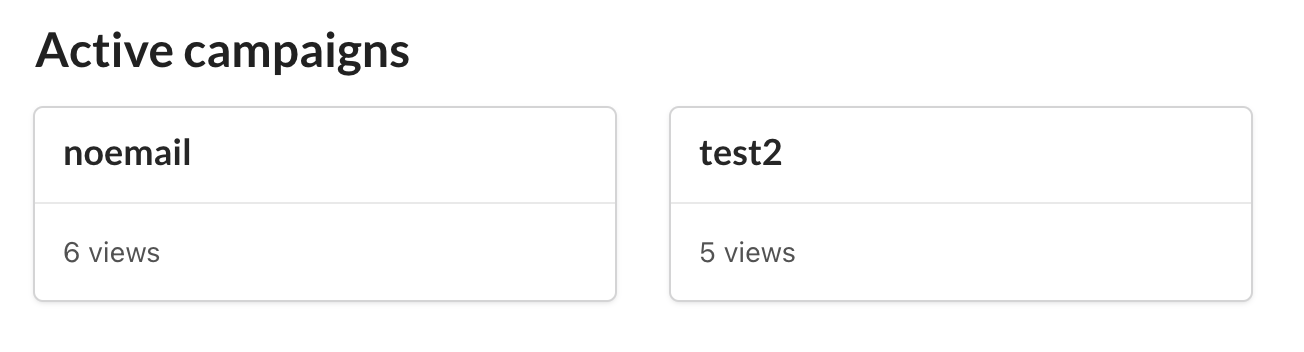
\includegraphics[width=0.8\textwidth]{images/active-campaigns.png}
\caption{List of active campaigns}
\end{figure}

\subsubsection{Campaign Details Page}

This page summarises the data collected about a certain campaign based on a campaign ID. It shows the total views, unique views (per email identifier that is passed in as a query parameter), and also the views per recipient.

\begin{figure}[H]
\centering
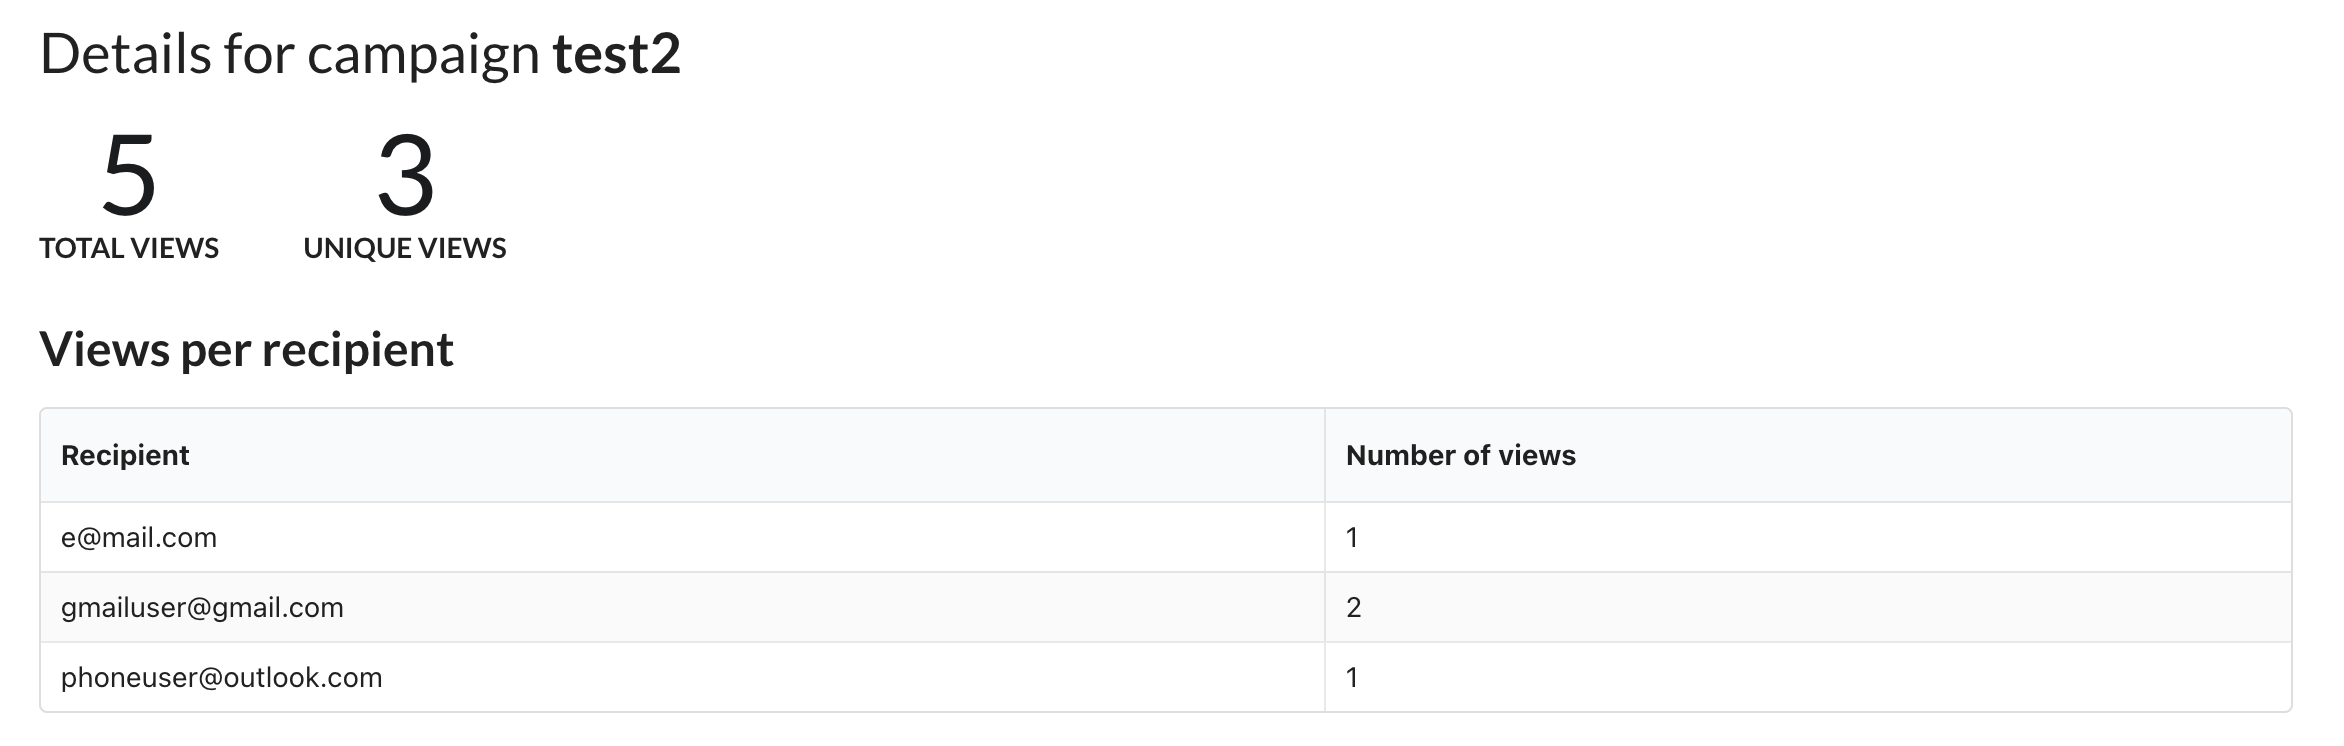
\includegraphics[width=0.8\textwidth]{images/summary-campaign.png}
\caption{Summary of all views collected from spy pixels with campaign ID \texttt{test2}}
\end{figure}

The logs are listed in chronological order, and can be expanded to show more information regarding the metadata collected when the spy pixel was loaded. Metadata includes the browser, device, OS and architecture extracted from the user agent, and also the country, city and IP address. Cookies are also scraped however I haven't encountered an email client that allows cookies to be scraped (this feature does work however if spy pixel is loaded in a new tab).

\begin{figure}[H]
\centering
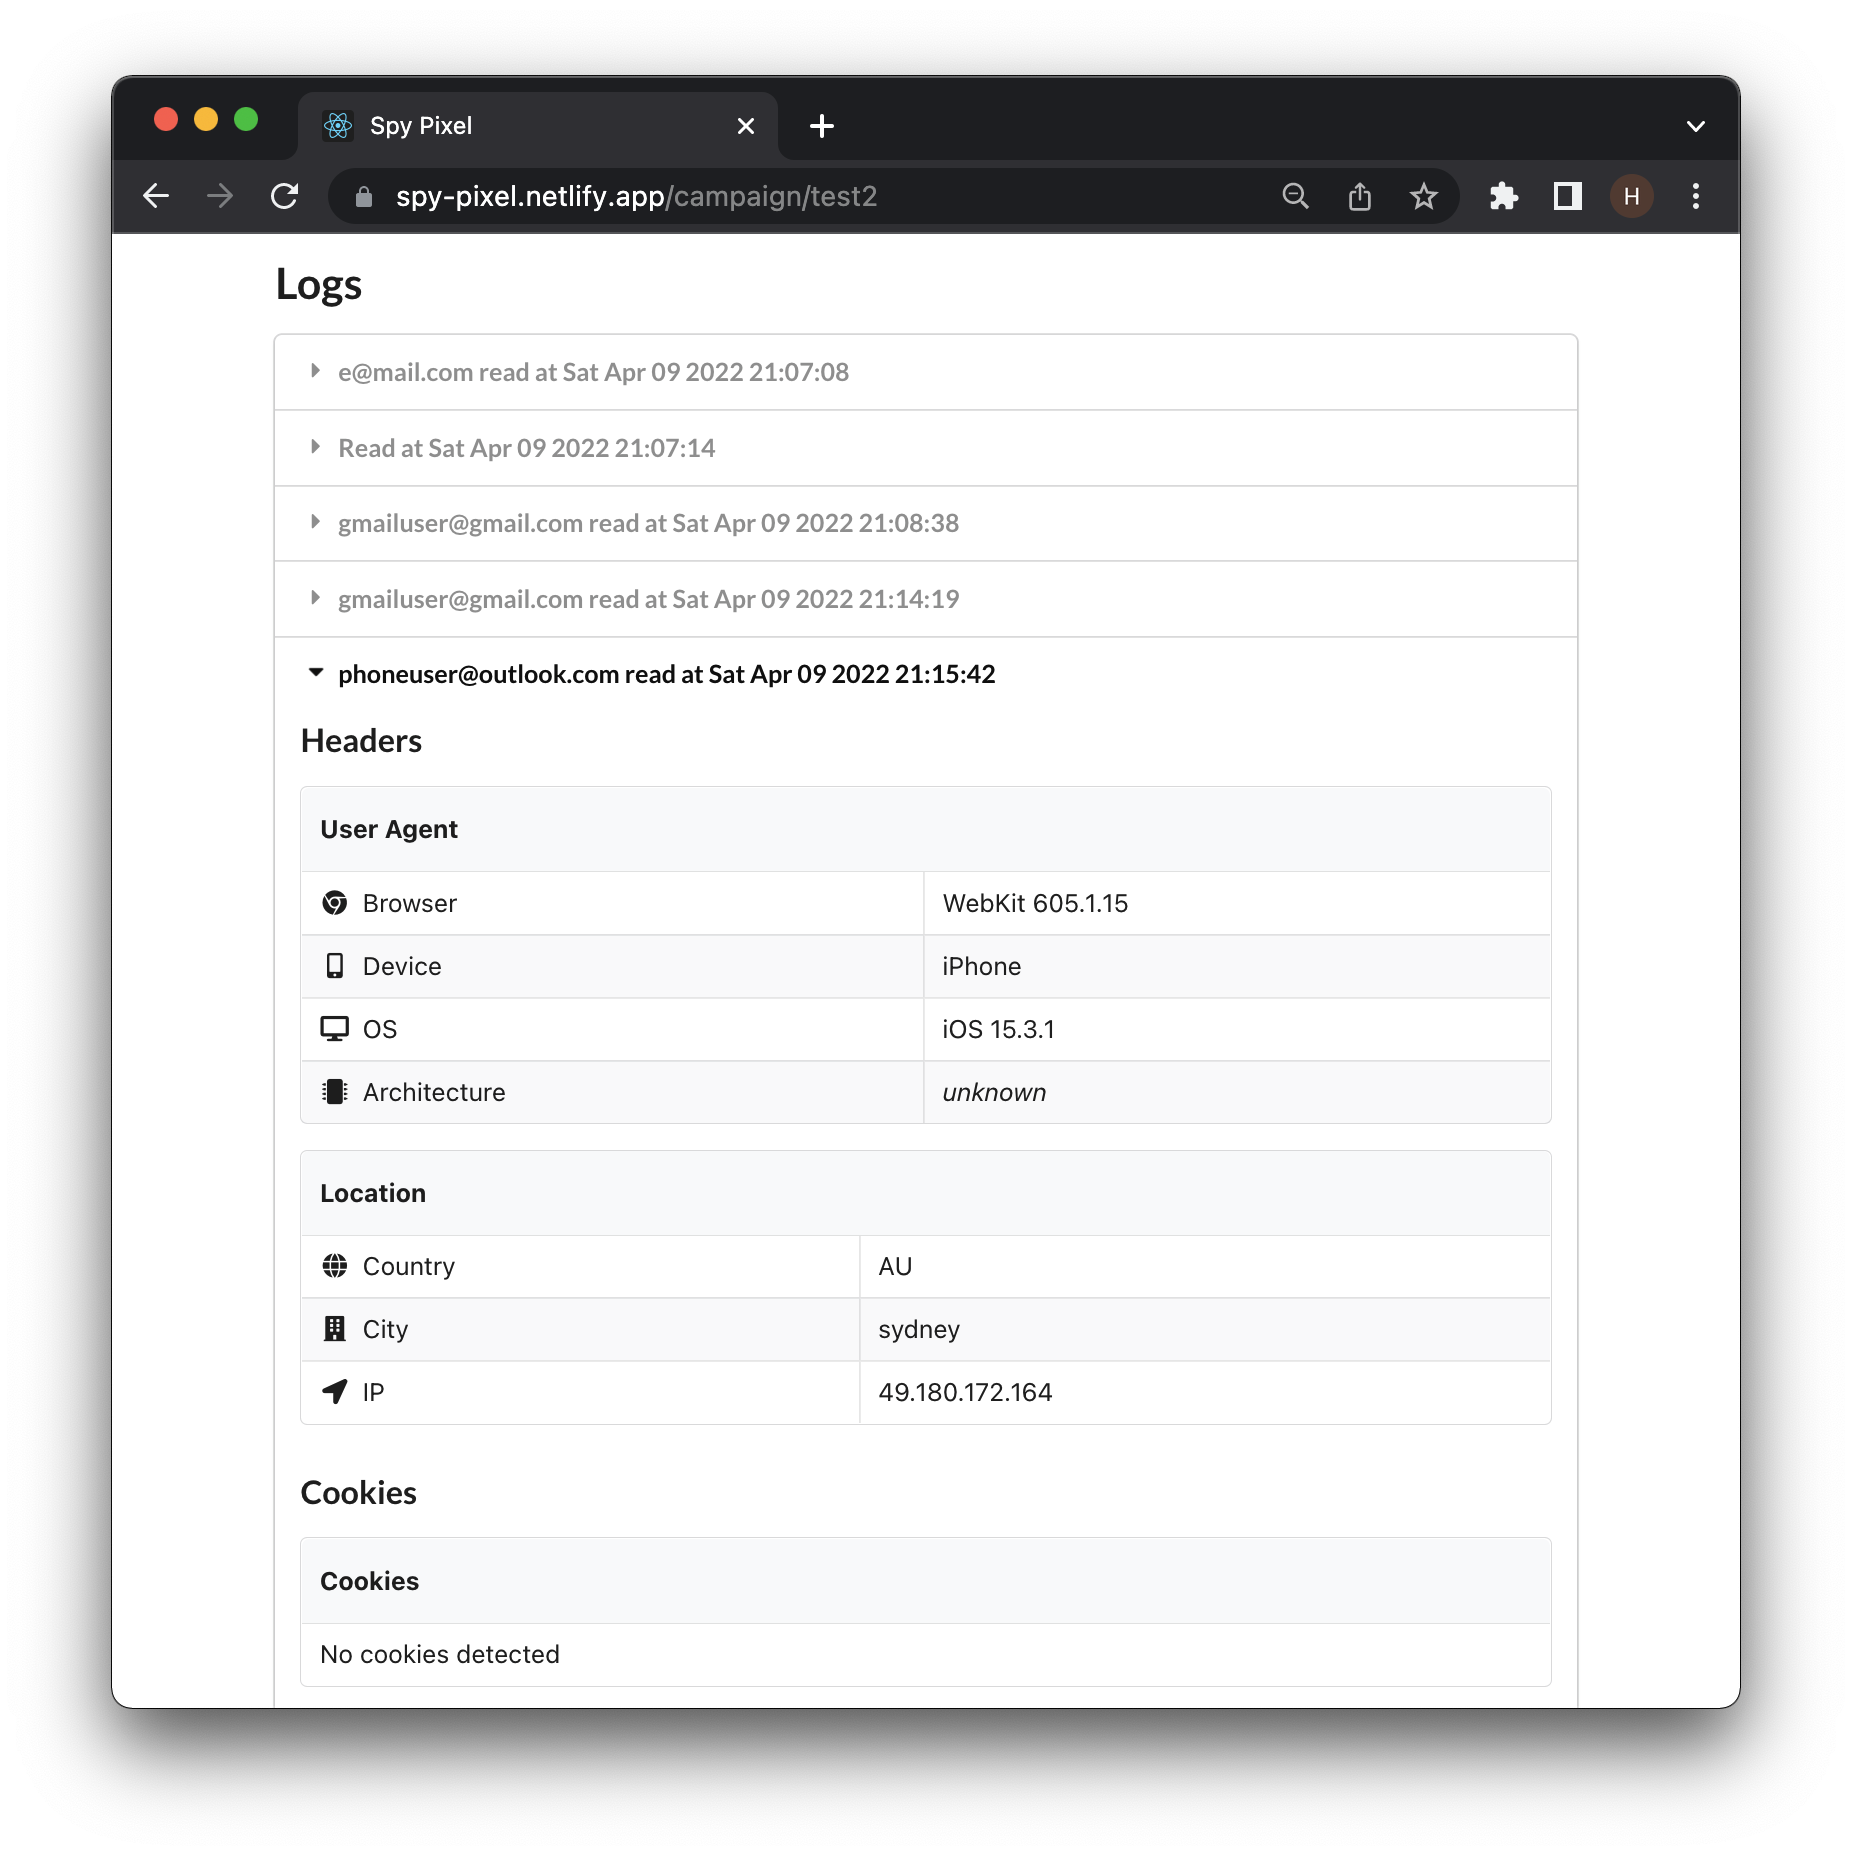
\includegraphics[width=0.7\textwidth]{images/logs.png}
\caption{Metadata shown in an easy-to-read table}
\end{figure}

If the spy pixel was loaded through a proxy, the proxy name is shown and can help explain nonsensical metadata (such as a ZZ country!).

\begin{figure}[H]
\centering
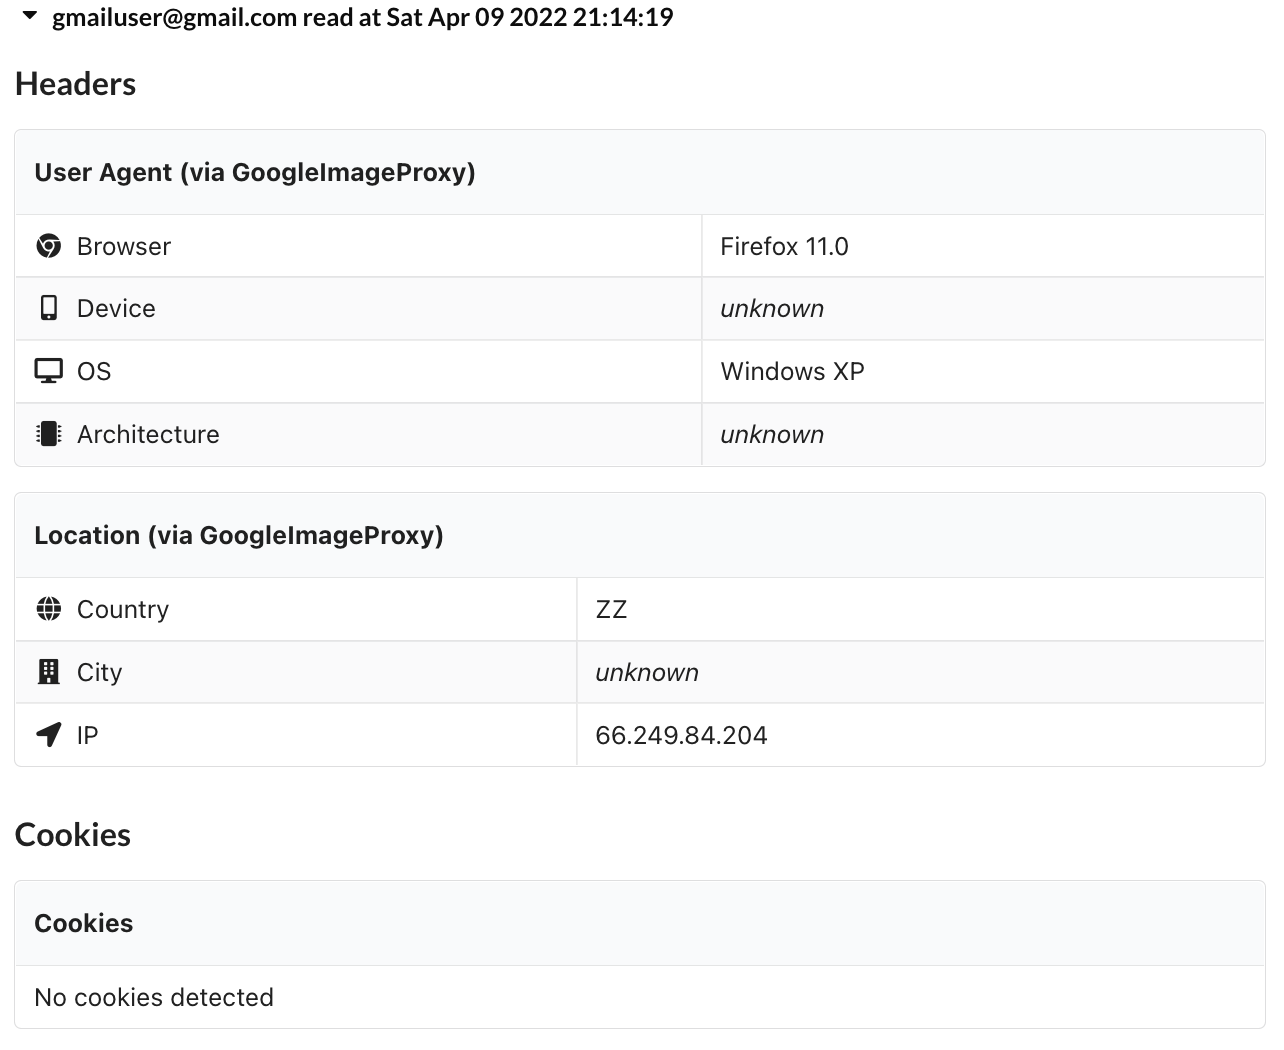
\includegraphics[width=0.5\textwidth]{images/gmailproxy.png}
\caption{Detection of GoogleImageProxy}
\end{figure}

\section{An aside - HTML in Emails}

While inspecting the HTML in emails, you might notice two odd things: inline styling is used everywhere, and data table tags \texttt{table}, \texttt{tbody}, \texttt{td} and \texttt{tr} are used in place of \texttt{div}s and other HTML elements. Below is a UNSW newsletter email with its HTML shown next to it.

\begin{figure}[H]
    \centering
    \subfloat[\centering Email's HTML with inline styling and table tags]{{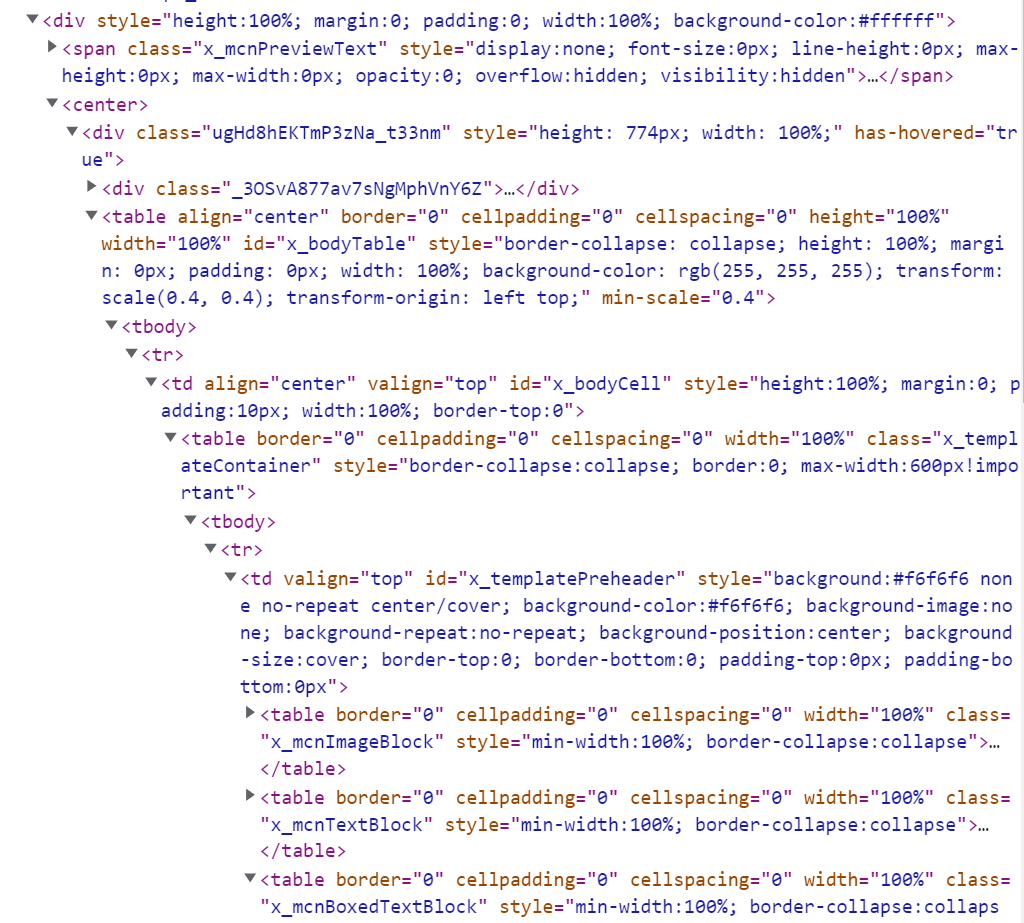
\includegraphics[width=0.5\textwidth]{images/htmlinspectedemail.png} }}
    \qquad
    \subfloat[\centering Rendered email]{{
\includegraphics[width=0.4\textwidth]{images/unswlaunchyourcareer.png} }}
    \caption{HTML contains tables, yet the original email has no data tables visible}
\end{figure}

It turns out that emails have to use HTML like this because of the restrictions of email clients. Email clients are old school, meaning they haven't changed much since their introduction. Emails are also rendered statically, not dynamically like a React website, meaning they aren't able to respond to user input and change its content. Due to the multitude of screen sizes, browsers, devices and email clients there are available, there are over 15000 ways an email can be rendered (an accuracy check can be found in Appendix \ref{appendix-number-of-ways-to-render-email}). In other words, there are 15000 ways to parse an HTML document, and so HTML must be written in a way that even the most basic email client can render an email exactly as the sender intended.

For example, some email clients strip away \texttt{<head>} when rendering the email, taking away with it the style sheets. Not only does this explain the overbearing presence of inline styling, but also why emails don't tend to use non-browser friendly fonts that you would typically be able to load with a CSS style sheet.

Some email clients also don't render \texttt{div} blocks properly, and can only render \texttt{table}s. To ensure the layout is preserved across all email clients, senders must use \texttt{table}, \texttt{tr} and \texttt{td} to format the contents of the email.

HTML is also rendered from top to bottom, just like HTML in the web. To ensure email's content is loaded quickly, the spy pixel should be placed at the bottom of the email.

\section{Reflection}

I'm really grateful to have the opportunity to learn what I did! It's not everyday that my university projects spark so much curiosity and freedom for me to explore and learn what I want to explore and learn.

As explained in section \ref{context}, I chose this topic because I noticed privacy concerns when using the mass email service GMass and I was able to see each time my recipients viewed my email. Initially I thought emails were simple forms of communication, much like a digital letter that only contained its content, but now that I've discovered the existence of spy pixels, it's clear to me that even emails have been "weaponised" as tools to track and collect data on users, whether they like it or not.

I consider myself very lucky to have chosen this topic to research on, because I am now quite wary of spy pixels and have taken strategies to prevent their effect. Whereever possible, I try and use Chrome on my laptop or PC to browse my emails since I have downloaded the Chrome extension \href{https://chrome.google.com/webstore/detail/pixelblock/jmpmfcjnflbcoidlgapblgpgbilinlem?hl=en}{PixelBlock} which is most effective at preventing spy pixels. When I'm out, I only use GMail on my phone since it uses GoogleImageProxy to anonymise my data.

The learning experience has also changed how quickly I reply to my emails. Recently, I've been applying for internships, and chances are that if they use an automated email service to send me emails, they've probably seen that I've read the email already. To show companies I am an attentive person, I reply as quickly as I can!

I faced a multitude of challenges during the completion of my assignment. I work full time meaning I needed to balance my study sessions and university courses around my 9-5 work schedule. Another major external factor that implicated me was having to travel two hours each day to Gosford Hospital from weeks 6 to 8.

There were also a few technical challenges. Google Cloud App Engine was more overwhelming than I thought, and I had initially started on Google Cloud Functions which later turned out to be the wrong microservice to use. The process involved a lot of googling and debugging, and managed to get it working on Google Cloud App Engine on my second day of trying! If I had to do this again, I would just use Heroku since I had experience with it, but I was stubborn and wanted to save my deeply-sunk cost. At least now I have been exposed to GCP at a basic level.

Another problem I faced was React upgrading to version 18 on 29 March 2022. This was not backwards compatible with my libraries, and I went through a deep rabbit hole of reinstalling \texttt{webpack} and \texttt{npm}, before finding the root cause! Looking back, if I had just started my assignment earlier I wouldn't have ran into this problem, but another lesson that I learnt is to always inspect my \texttt{package.json} file and look carefully at my dependency versions.

I also tried to use \texttt{geoip-lite} to obtain a geolocation based on an IP address. While this seemed like a good idea, a few google searches revealed that IP addresses and physical addresses aren't as relatable as I thought. An IP address is the address of a computer in a network and not in real life, which explained why most IP addresses I tested with ended up showing the data centre in Sydney's CBD. This was a minor setback since I thought this feature would be super impressive, but had to quickly change scope once I realised I didn't have enough information to pull it off.

Overall I'm quite proud of my project! It is a fully working demo of how spy pixels work, and even has a frontend to be a service other people can use. I was also able to further my learning by finding differences between HTML in emails and HTML on the web, which revealed just how outdated emails and backwards compatible emails aim to be. If I had more time, perhaps I could have implemented a feature for users to upload their own image and have that image log views. This would make it obvious that it's not just transparent pixels we need to be worried about, but the actual process of loading any image in our emails.

\section{Conclusion}

Spy pixels take advantage of the most fundamental rules of HTML image rendering to track email recipients. It's a tool that not only tracks email reads, but user metadata including their browser, device, OS, architecture, country, city, IP address, and cookies. This makes the collected data extremely valuable for marketing teams of companies who send frequent email newsletters, as they can see how effective their emails are and how changes in marketing strategies impact user interaction.

Unlike other data gathering tools, spy pixels secretly collect this information without notifying the user, since they are transparent and small. They can also come in the form of large visible images, since it is the process of loading an image off an external server that allows user's metadata to be collected. Out of all the email browsers that I've tested with, I believe GMail to be the best service to use to maintain your anonymity since it loads images through a proxy, anonymising the data in the request when the email is loaded. This doesn't prevent a request from being logged and notifying the sender that you've seen their email, but makes it so that the metadata sent cannot identify the recipient.

\newpage

\section{Appendix}

\subsection{\label{appendix-inbox}Spy pixels in my inbox}

\begin{figure}[H]
\centering
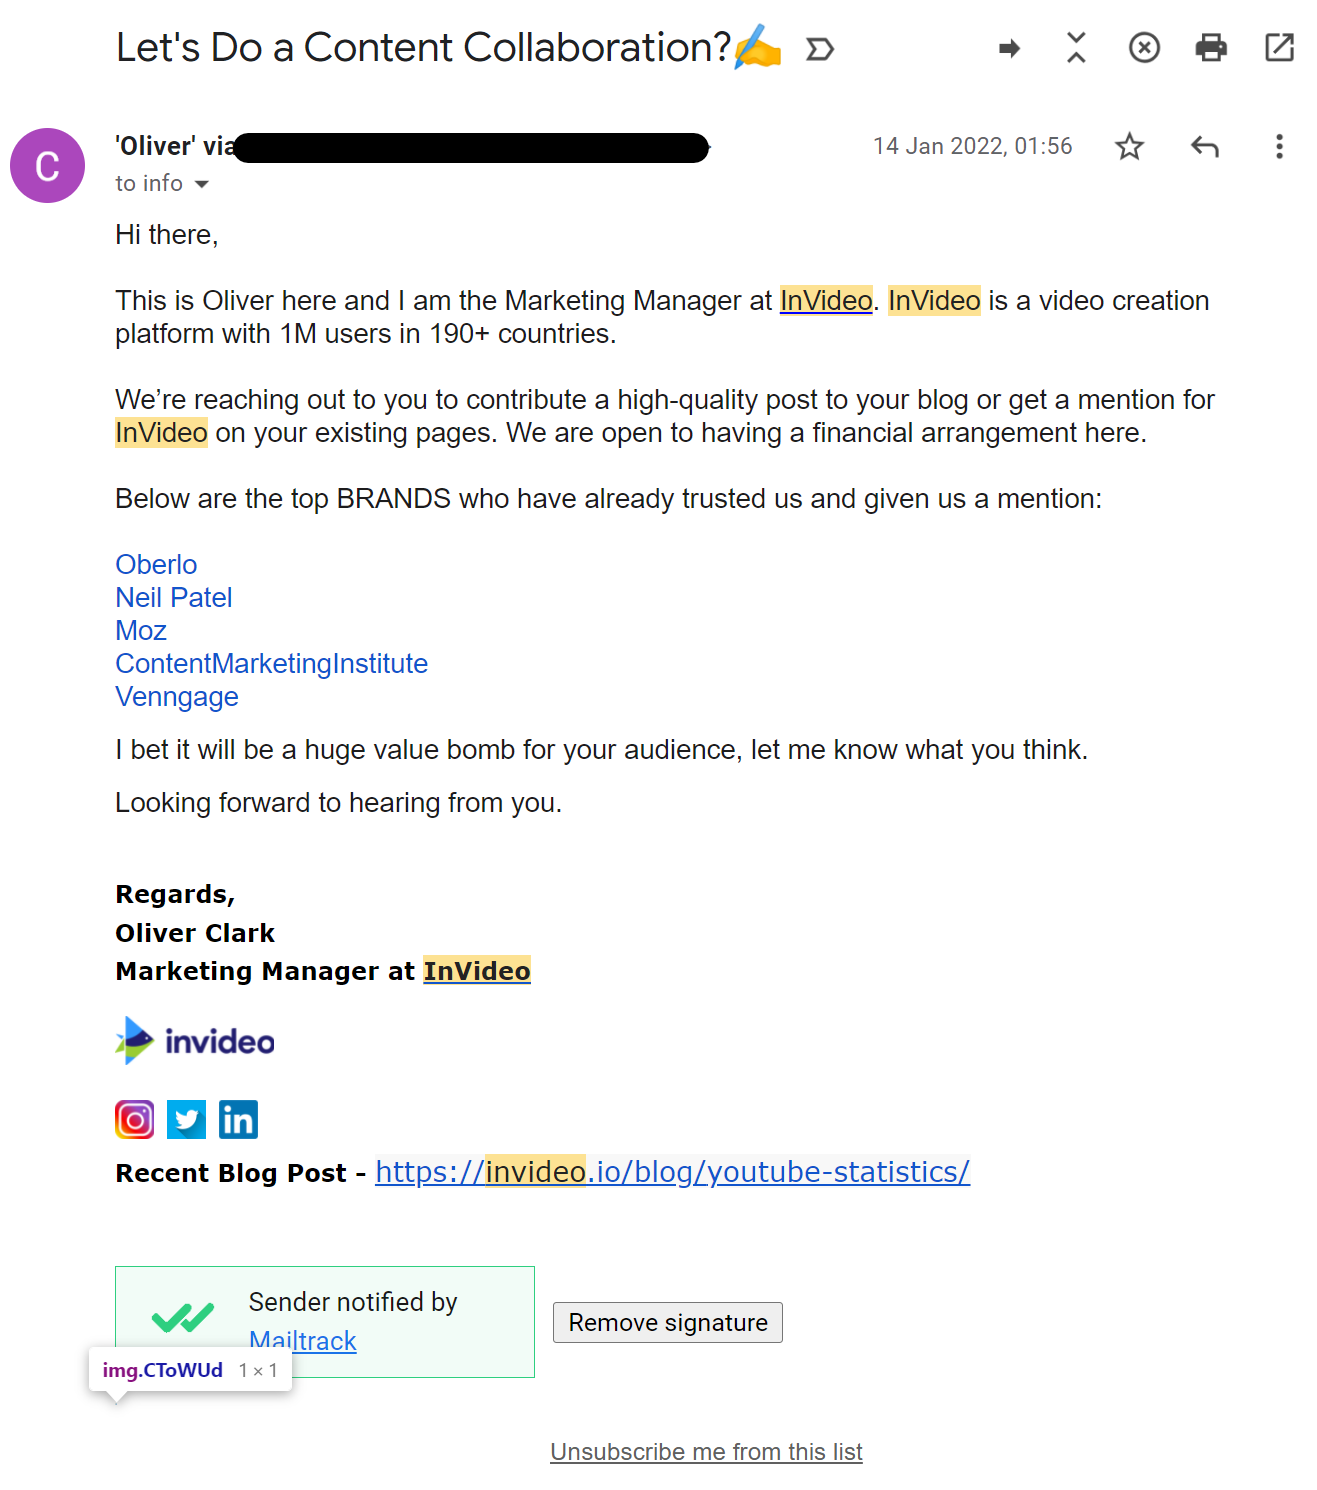
\includegraphics[width=0.8\textwidth]{images/oliver.png}
\caption{\label{oliver}Mailtrack embeds a spy pixel at the bottom. Luckily they are nice enough to tell me about it!}
\end{figure}

\begin{figure}[H]
    \centering
    \subfloat[\centering Glue embeds a spy pixel at the top]{{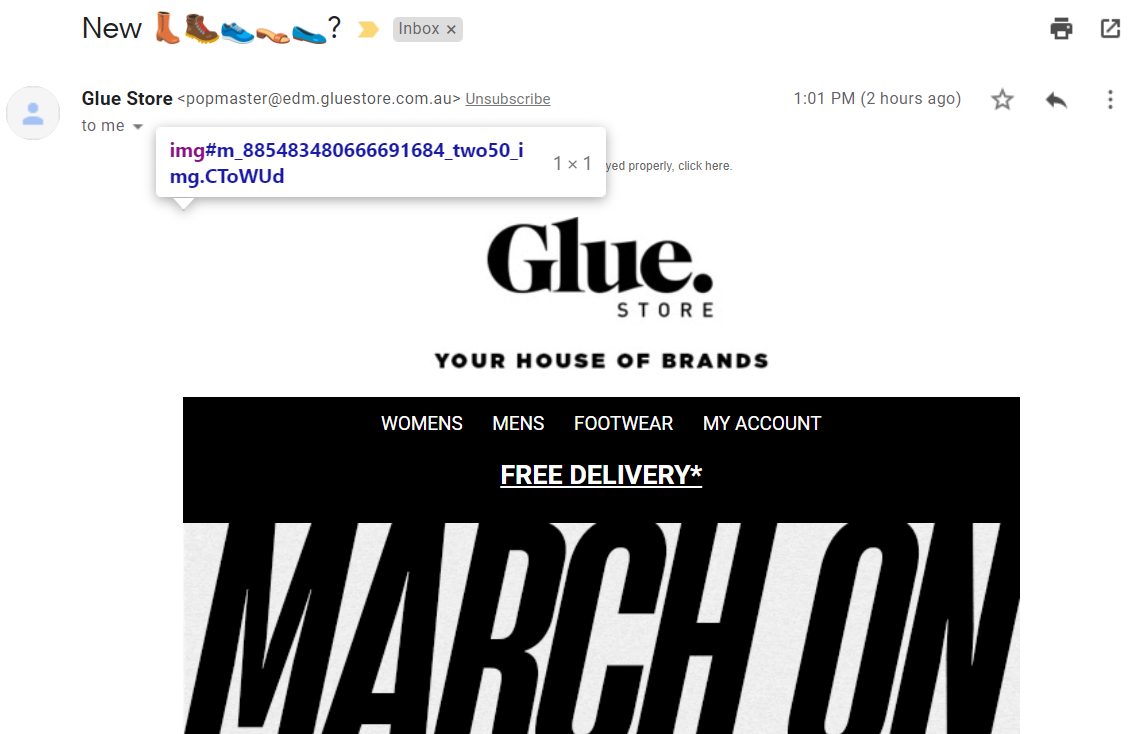
\includegraphics[width=0.4\textwidth]{images/glue_top.png} }}
    \qquad
    \subfloat[\centering Glue embeds a second spy pixel at the bottom]{{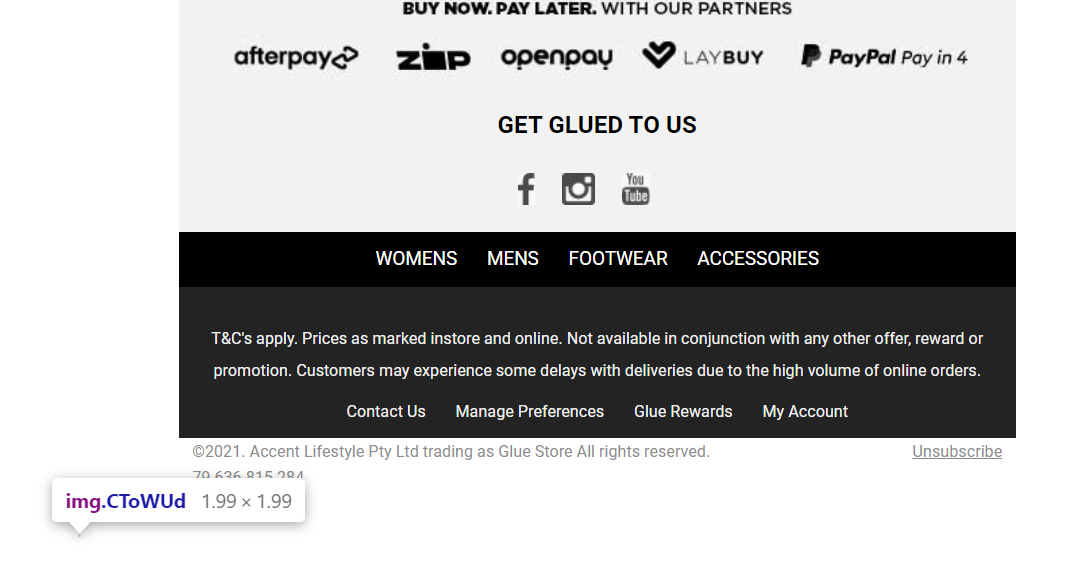
\includegraphics[width=0.4\textwidth]{images/glue_bot.png} }}
    \caption{Glue embeds two spy pixels in their email}
\end{figure}

\subsection{\label{appendix-backend-code}Backend code}

\href{https://github.com/hayeselnut/spy-pixel/tree/main/backend}{\texttt{https://github.com/hayeselnut/spy-pixel/tree/main/backend}}

\subsubsection{Spy pixel route}

\begin{python}
@app.route('/spy-pixel.gif')
def spy_pixel():
    # We don't want to log our own views
    if request.headers.get("Referer") != "https://mail.google.com/" and request.headers.get("Referer") != "https://spy-pixel.netlify.app/":
        # Campaign is loggable
        if request.args.get("campaign"):
            # Log to database
            log = {
                u'timestamp': datetime.datetime.now(),
                u'email': request.args.get("email"),
                u'headers': dict(request.headers),
                u'cookies': dict(request.cookies)
            }

            doc_ref = db.collection(u'campaigns').document(request.args.get("campaign"))
            doc = doc_ref.get()

            if not doc.exists:
                doc_ref.set({u'logs': []})

            doc_ref.update({u'logs': firestore.ArrayUnion([log])})

    gif_str = base64.b64decode('R0lGODlhAQABAIAAAP///////yH5BAEKAAEALAAAAAABAAEAAAICTAEAOw==')
    resp = make_response(send_file(io.BytesIO(gif_str), mimetype='image/gif'), 200)
    return resp
\end{python}

\subsection{\label{appendix-frontend-code}Frontend code}

\href{https://github.com/hayeselnut/spy-pixel/tree/main/frontend}{\texttt{https://github.com/hayeselnut/spy-pixel/tree/main/frontend}}

\subsection{\label{appendix-number-of-ways-to-render-email}Are there really 15000 ways to render an email?}

\subsubsection{Online email clients}

There \textbf{110 common web browsers} (according to \href{https://www.npmjs.com/package/ua-parser-js}{\texttt{ua-parser-js}}): 2345Explorer, 360 Browser, Amaya, Android Browser, Arora, Avant, Avast, AVG,
BIDUBrowser, Baidu, Basilisk, Blazer, Bolt, Brave, Bowser, Camino, Chimera,
Chrome Headless, Chrome WebView, Chrome, Chromium, Comodo Dragon, Dillo,
Dolphin, Doris, Edge, Electron, Epiphany, Facebook, Falkon, Fennec, Firebird,
Firefox [Reality], Flock, Flow, GSA, GoBrowser, ICE Browser, IE, IEMobile, IceApe, 
IceCat, IceDragon, Iceweasel, Instagram, Iridium, Iron, Jasmine, K-Meleon,
Kindle, Klar, Konqueror, LBBROWSER, Line, Links, Lunascape, Lynx, MIUI Browser,
Maemo Browser, Maemo, Maxthon, MetaSr Midori, Minimo, Mobile Safari, Mosaic,
Mozilla, NetFront, NetSurf, Netfront, Netscape, NokiaBrowser, Obigo, Oculus Browser,
OmniWeb, Opera Coast, Opera [Mini/Mobi/Tablet], PaleMoon, PhantomJS, Phoenix, 
Polaris, Puffin, QQ, QQBrowser, QQBrowserLite, Quark, QupZilla, RockMelt, Safari, 
Sailfish Browser, Samsung Browser, SeaMonkey, Silk, Skyfire, Sleipnir, Slim, 
SlimBrowser, Swiftfox, Tesla, Tizen Browser, UCBrowser, UP.Browser, Vivaldi, 
Waterfox, WeChat, Weibo, Yandex, baidu, iCab, w3m, Whale Browser

There are at least \textbf{6 common online email clients}: GMail, Hotmail, Yahoo! Mail, ProtonMail, Outlook, iCloud Mail.

Let us assume there are \textbf{10 different screen sizes} browser windows can take. Realistically, this is almost an infinite number, so this is a conservative estimate.

Altogether, there are $\mathbf{110 \times 6 \times 10 = 6600}$ different ways to render an email on an online email client.

\subsubsection{Email apps on devices}

There are \textbf{49 common vendors of devices} (according to \href{https://www.npmjs.com/package/ua-parser-js}{\texttt{ua-parser-js}}): Acer, Alcatel, Amazon, Apple, Archos, ASUS, AT\&T, BenQ, BlackBerry, Dell,
Essential, Fairphone, GeeksPhone, Google, HP, HTC, Huawei, Jolla, Lenovo, LG, 
Meizu, Microsoft, Motorola, Nexian, Nintendo, Nokia, Nvidia, OnePlus, OPPO, Ouya,
Palm, Panasonic, Pebble, Polytron, Realme, RIM, Roku, Samsung, Sharp, Siemens,
Sony[Ericsson], Sprint, Tesla, Vivo, Vodafone, Xbox, Xiaomi, Zebra, ZTE.

Let us assume that on average, each vendor listed above has at least \textbf{10 different device models} that can browse the internet. This is a conservative estimate since some vendors have many, many devices. For example, Apple has over 30 iPhone and iPad models altogether, and Samsung has over 50.

Let us assume that there are at least \textbf{20 email apps} that can be downloaded onto each device model. There are actually over 100 email apps in both App Store and Google Play, but we shall make a conservative estimation since some devices such as Blackberry and Nintendo don't have that many number of choices.

Altogether, there are $\mathbf{49 \times 10 \times 20 = 9800}$ different ways emails can be natively rendered on a device.

\subsubsection{Conclusion}

Altogether, there are $\mathbf{6600 + 9800 = 16400}$ different ways to render an email, and this is using conservative estimates throughout.

\subsection{\label{blogs}Blog Posts}

\paragraph{23 Feb 2022} \href{https://www.openlearning.com/u/hayeschoy-r7a9ti/blog/SomethingAwesomeEmailSecurity/}{Email Security}
\paragraph{3 Mar 2022} \href{https://www.openlearning.com/u/hayeschoy-r7a9ti/blog/SomethingAwesomeResearch3March/}{Research}
\paragraph{10 Mar 2022} \href{https://www.openlearning.com/u/hayeschoy-r7a9ti/blog/SomethingAwesomeCheckingMyOwnInbox10March/}{Checking My Own Inbox}
\paragraph{22 Mar 2022} \href{https://www.openlearning.com/u/hayeschoy-r7a9ti/blog/SomethingAwesomeHtmlInEmails22March/}{HTML In Emails}
\paragraph{31 Mar 2022} \href{https://www.openlearning.com/u/hayeschoy-r7a9ti/blog/SomethingAwesomeFirstPrototype/}{First Prototype}
\paragraph{6 Apr 2022} \href{https://www.openlearning.com/u/hayeschoy-r7a9ti/blog/SomethingAwesomeDatabaseIntegration/}{Database Integration}
\paragraph{7 Apr 2022} \href{https://www.openlearning.com/u/hayeschoy-r7a9ti/blog/SomethingAwesomeFrontendDeployed/}{Frontend Deployed}

\subsection{\label{blogs}Estimated hours of work}

\begin{center}
\begin{tabular}{ |m{0.3\textwidth}|l|m{0.6\textwidth}| }
    \hline
    \textbf{Activity} & \textbf{Hours} & \textbf{Notes} \\ 
    \hline\hline
    Deciding project & 1 & Blog post \href{https://www.openlearning.com/u/hayeschoy-r7a9ti/blog/SomethingAwesomeEmailSecurity/}{Email Security} \\  
    \hline
    Researching spy pixels & 1 & Blog post \href{https://www.openlearning.com/u/hayeschoy-r7a9ti/blog/SomethingAwesomeResearch3March/}{Research} \\
    \hline
    Looking at my inbox & 1 & Blog post \href{https://www.openlearning.com/u/hayeschoy-r7a9ti/blog/SomethingAwesomeCheckingMyOwnInbox10March/}{Checking My Own Inbox} \\
    \hline
    Researching HTML in emails & 1 & Blog post \href{https://www.openlearning.com/u/hayeschoy-r7a9ti/blog/SomethingAwesomeHtmlInEmails22March/}{HTML In Emails} \\
    \hline
    First prototype & 2 &  \\
    \hline
    Deploying prototype to Google Cloud App Engine & 5 & Blog post \href{https://www.openlearning.com/u/hayeschoy-r7a9ti/blog/SomethingAwesomeFirstPrototype/}{First Prototype} \\
    \hline
    Firestore Database local integration & 1 & Blog post \href{https://www.openlearning.com/u/hayeschoy-r7a9ti/blog/SomethingAwesomeDatabaseIntegration/}{Database Integration} \\
    \hline
    Firestore Database integration with deployed backend & 4 & \\
    \hline
    Configuring React & 2 & Unbeknownst to me, React 18 was released on 29 March 2022, which was not backwards compatible with my libraries. I went through a deep rabbit hole of reinstalling \texttt{webpack} and \texttt{npm}, before finding the root cause. \\
    \hline
    Frontend development & 8 &  \\
    \hline
    Frontend deployment & 2 & Blogpost \href{https://www.openlearning.com/u/hayeschoy-r7a9ti/blog/SomethingAwesomeFrontendDeployed/}{Frontend Deployed} \newline GitHub Pages didn't work, so after a lots of debugging, decided to learn and use Netlify instead \\
    \hline
    Debug and clean & 3 & Changing icons, fixing backend logging unwanted views where referer was definitely the user \\
    \hline
    Report Writing & 6 & \\   
    \hline\hline
    
    \textbf{Total} & \textbf{37} & \\
    \hline
\end{tabular}
\end{center}

% \begin{center}
% \begin{tabular}{ | m{5em} | m{1cm}| m{1cm} | } 
%   \hline
%   cell1 dummy text dummy text dummy text& cell2 & cell3 \\ 
%   \hline
%   cell1 dummy text dummy text dummy text & cell5 & cell6 \\ 
%   \hline
%   cell7 & cell8 & cell9 \\ 
%   \hline
% \end{tabular}
% \end{center}

\section{Further Reading}

\subsection{Spy pixels}

\begin{itemize}
  \item \href{https://www.theverge.com/2019/7/3/20681508/tracking-pixel-email-spying-superhuman-web-beacon-open-tracking-read-receipts-location}{https://www.theverge.com/2019/7/3/20681508/tracking-pixel-email-spying-superhuman-web-beacon-open-tracking-read-receipts-location}
  \item \href{https://www.nutshell.com/blog/email-tracking-pixels-101-how-do-tracking-pixels-work}{https://www.nutshell.com/blog/email-tracking-pixels-101-how-do-tracking-pixels-work}
  \item \href{https://www.wired.com/story/how-to-tell-which-emails-track-you/}{https://www.wired.com/story/how-to-tell-which-emails-track-you/}
  \item \href{https://mashable.com/article/how-to-block-email-pixel-tracking}{https://mashable.com/article/how-to-block-email-pixel-tracking}

  \item \href{http://engineering.curalate.com/2016/10/19/building-a-tracking-pixel.html}{http://engineering.curalate.com/2016/10/19/building-a-tracking-pixel.html}
  \item \href{https://limjiahe.com/2020/06/20/how-1x1-pixel-tracking-cookies-work-learn-by-implementing-your-own-tracking-system/}{https://limjiahe.com/2020/06/20/how-1x1-pixel-tracking-cookies-work-learn-by-implementing-your-own-tracking-system/}
  \item \href{https://www.youtube.com/watch?v=k4HImDV9S2Y}{https://www.youtube.com/watch?v=k4HImDV9S2Y}
\end{itemize}

\subsection{HTML in emails}

\begin{itemize}
  \item \href{https://www.htmlemailcheck.com/check/}{https://www.htmlemailcheck.com/check/}
  \item \href{https://www.smashingmagazine.com/2017/01/introduction-building-sending-html-email-for-web-developers/}{https://www.smashingmagazine.com/2017/01/introduction-building-sending-html-email-for-web-developers/}
  \item \href{https://blog.hubspot.com/marketing/html-email}{https://blog.hubspot.com/marketing/html-email}
  \item \href{https://mailbakery.com/blog/how-email-html-coding-differs-from-web-html-coding/}{https://mailbakery.com/blog/how-email-html-coding-differs-from-web-html-coding/}
  \item \href{https://www.campaignmonitor.com/dev-resources/guides/coding-html-emails/}{https://www.campaignmonitor.com/dev-resources/guides/coding-html-emails/}
\end{itemize}

\end{document}